% Created by tikzDevice version 0.12.6 on 2026-07-09 15:42:27
% !TEX encoding = UTF-8 Unicode
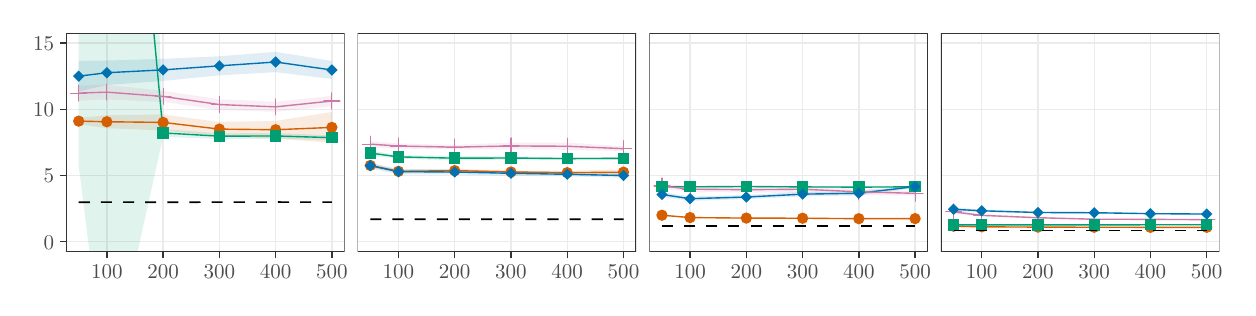
\begin{tikzpicture}[x=1pt,y=1pt]
\definecolor{fillColor}{RGB}{255,255,255}
\path[use as bounding box,fill=fillColor,fill opacity=0.00] (0,0) rectangle (433.62, 93.95);
\begin{scope}
\path[clip] (  0.00,  0.00) rectangle (433.62, 93.95);
\definecolor{drawColor}{RGB}{255,255,255}
\definecolor{fillColor}{RGB}{255,255,255}

\path[draw=drawColor,line width= 0.5pt,line join=round,line cap=round,fill=fillColor] ( -0.00,  0.00) rectangle (433.62, 93.95);
\end{scope}
\begin{scope}
\path[clip] ( 13.87, 12.99) rectangle (114.50, 91.95);
\definecolor{fillColor}{RGB}{255,255,255}

\path[fill=fillColor] ( 13.87, 12.99) rectangle (114.50, 91.95);
\definecolor{drawColor}{gray}{0.92}

\path[draw=drawColor,line width= 0.5pt,line join=round] ( 13.87, 16.58) --
	(114.50, 16.58);

\path[draw=drawColor,line width= 0.5pt,line join=round] ( 13.87, 40.52) --
	(114.50, 40.52);

\path[draw=drawColor,line width= 0.5pt,line join=round] ( 13.87, 64.47) --
	(114.50, 64.47);

\path[draw=drawColor,line width= 0.5pt,line join=round] ( 13.87, 88.42) --
	(114.50, 88.42);

\path[draw=drawColor,line width= 0.5pt,line join=round] ( 28.61, 12.99) --
	( 28.61, 91.95);

\path[draw=drawColor,line width= 0.5pt,line join=round] ( 48.94, 12.99) --
	( 48.94, 91.95);

\path[draw=drawColor,line width= 0.5pt,line join=round] ( 69.27, 12.99) --
	( 69.27, 91.95);

\path[draw=drawColor,line width= 0.5pt,line join=round] ( 89.60, 12.99) --
	( 89.60, 91.95);

\path[draw=drawColor,line width= 0.5pt,line join=round] (109.92, 12.99) --
	(109.92, 91.95);
\definecolor{fillColor}{RGB}{213,94,0}

\path[fill=fillColor,fill opacity=0.12] ( 18.45, 61.31) --
	( 28.61, 62.30) --
	( 48.94, 62.57) --
	( 69.27, 59.91) --
	( 89.60, 60.26) --
	(109.92, 63.48) --
	(109.92, 52.34) --
	( 89.60, 53.87) --
	( 69.27, 54.68) --
	( 48.94, 56.84) --
	( 28.61, 57.62) --
	( 18.45, 59.05) --
	cycle;

\path[] ( 18.45, 61.31) --
	( 28.61, 62.30) --
	( 48.94, 62.57) --
	( 69.27, 59.91) --
	( 89.60, 60.26) --
	(109.92, 63.48);

\path[] (109.92, 52.34) --
	( 89.60, 53.87) --
	( 69.27, 54.68) --
	( 48.94, 56.84) --
	( 28.61, 57.62) --
	( 18.45, 59.05);
\definecolor{fillColor}{RGB}{0,158,115}

\path[fill=fillColor,fill opacity=0.12] ( 18.45,149.62) --
	( 28.61,589.39) --
	( 48.94, 57.30) --
	( 69.27, 55.78) --
	( 89.60, 55.83) --
	(109.92, 55.09) --
	(109.92, 53.32) --
	( 89.60, 53.81) --
	( 69.27, 53.70) --
	( 48.94, 54.53) --
	( 28.61,-37.04) --
	( 18.45, 44.02) --
	cycle;

\path[] ( 18.45,149.62) --
	( 28.61,589.39) --
	( 48.94, 57.30) --
	( 69.27, 55.78) --
	( 89.60, 55.83) --
	(109.92, 55.09);

\path[] (109.92, 53.32) --
	( 89.60, 53.81) --
	( 69.27, 53.70) --
	( 48.94, 54.53) --
	( 28.61,-37.04) --
	( 18.45, 44.02);
\definecolor{fillColor}{RGB}{0,114,178}

\path[fill=fillColor,fill opacity=0.12] ( 18.45, 81.93) --
	( 28.61, 82.09) --
	( 48.94, 82.67) --
	( 69.27, 83.62) --
	( 89.60, 85.20) --
	(109.92, 81.93) --
	(109.92, 75.40) --
	( 89.60, 77.88) --
	( 69.27, 76.70) --
	( 48.94, 74.73) --
	( 28.61, 73.24) --
	( 18.45, 70.91) --
	cycle;

\path[] ( 18.45, 81.93) --
	( 28.61, 82.09) --
	( 48.94, 82.67) --
	( 69.27, 83.62) --
	( 89.60, 85.20) --
	(109.92, 81.93);

\path[] (109.92, 75.40) --
	( 89.60, 77.88) --
	( 69.27, 76.70) --
	( 48.94, 74.73) --
	( 28.61, 73.24) --
	( 18.45, 70.91);
\definecolor{fillColor}{RGB}{204,121,167}

\path[fill=fillColor,fill opacity=0.12] ( 18.45, 73.05) --
	( 28.61, 73.24) --
	( 48.94, 71.11) --
	( 69.27, 68.10) --
	( 89.60, 67.18) --
	(109.92, 69.33) --
	(109.92, 65.57) --
	( 89.60, 63.51) --
	( 69.27, 64.25) --
	( 48.94, 67.12) --
	( 28.61, 68.07) --
	( 18.45, 67.58) --
	cycle;

\path[] ( 18.45, 73.05) --
	( 28.61, 73.24) --
	( 48.94, 71.11) --
	( 69.27, 68.10) --
	( 89.60, 67.18) --
	(109.92, 69.33);

\path[] (109.92, 65.57) --
	( 89.60, 63.51) --
	( 69.27, 64.25) --
	( 48.94, 67.12) --
	( 28.61, 68.07) --
	( 18.45, 67.58);
\definecolor{drawColor}{RGB}{213,94,0}

\path[draw=drawColor,line width= 0.5pt,line join=round] ( 18.45, 60.18) --
	( 28.61, 59.96) --
	( 48.94, 59.71) --
	( 69.27, 57.30) --
	( 89.60, 57.07) --
	(109.92, 57.91);
\definecolor{drawColor}{RGB}{0,158,115}

\path[draw=drawColor,line width= 0.5pt,line join=round] ( 18.45, 96.82) --
	( 28.61,276.17) --
	( 48.94, 55.92) --
	( 69.27, 54.74) --
	( 89.60, 54.82) --
	(109.92, 54.21);
\definecolor{drawColor}{RGB}{0,114,178}

\path[draw=drawColor,line width= 0.5pt,line join=round] ( 18.45, 76.42) --
	( 28.61, 77.67) --
	( 48.94, 78.70) --
	( 69.27, 80.16) --
	( 89.60, 81.54) --
	(109.92, 78.66);
\definecolor{drawColor}{RGB}{204,121,167}

\path[draw=drawColor,line width= 0.5pt,line join=round] ( 18.45, 70.32) --
	( 28.61, 70.65) --
	( 48.94, 69.11) --
	( 69.27, 66.17) --
	( 89.60, 65.34) --
	(109.92, 67.45);
\definecolor{fillColor}{RGB}{213,94,0}

\path[fill=fillColor] ( 18.45, 60.18) circle (  2.05);

\path[draw=drawColor,line width= 0.4pt,line join=round,line cap=round] ( 15.55, 70.32) -- ( 21.35, 70.32);

\path[draw=drawColor,line width= 0.4pt,line join=round,line cap=round] ( 18.45, 67.42) -- ( 18.45, 73.22);
\definecolor{fillColor}{RGB}{0,158,115}

\path[fill=fillColor] ( 16.40, 94.77) --
	( 20.50, 94.77) --
	( 20.50, 98.87) --
	( 16.40, 98.87) --
	cycle;
\definecolor{fillColor}{RGB}{0,114,178}

\path[fill=fillColor] ( 16.40, 76.42) --
	( 18.45, 78.47) --
	( 20.50, 76.42) --
	( 18.45, 74.37) --
	cycle;
\definecolor{fillColor}{RGB}{213,94,0}

\path[fill=fillColor] ( 28.61, 59.96) circle (  2.05);

\path[draw=drawColor,line width= 0.4pt,line join=round,line cap=round] ( 25.71, 70.65) -- ( 31.51, 70.65);

\path[draw=drawColor,line width= 0.4pt,line join=round,line cap=round] ( 28.61, 67.75) -- ( 28.61, 73.55);
\definecolor{fillColor}{RGB}{0,158,115}

\path[fill=fillColor] ( 26.56,274.12) --
	( 30.66,274.12) --
	( 30.66,278.22) --
	( 26.56,278.22) --
	cycle;
\definecolor{fillColor}{RGB}{0,114,178}

\path[fill=fillColor] ( 26.56, 77.67) --
	( 28.61, 79.72) --
	( 30.66, 77.67) --
	( 28.61, 75.61) --
	cycle;
\definecolor{fillColor}{RGB}{213,94,0}

\path[fill=fillColor] ( 48.94, 59.71) circle (  2.05);

\path[draw=drawColor,line width= 0.4pt,line join=round,line cap=round] ( 46.04, 69.11) -- ( 51.84, 69.11);

\path[draw=drawColor,line width= 0.4pt,line join=round,line cap=round] ( 48.94, 66.21) -- ( 48.94, 72.01);
\definecolor{fillColor}{RGB}{0,158,115}

\path[fill=fillColor] ( 46.89, 53.86) --
	( 50.99, 53.86) --
	( 50.99, 57.97) --
	( 46.89, 57.97) --
	cycle;
\definecolor{fillColor}{RGB}{0,114,178}

\path[fill=fillColor] ( 46.89, 78.70) --
	( 48.94, 80.75) --
	( 50.99, 78.70) --
	( 48.94, 76.65) --
	cycle;
\definecolor{fillColor}{RGB}{213,94,0}

\path[fill=fillColor] ( 69.27, 57.30) circle (  2.05);

\path[draw=drawColor,line width= 0.4pt,line join=round,line cap=round] ( 66.37, 66.17) -- ( 72.17, 66.17);

\path[draw=drawColor,line width= 0.4pt,line join=round,line cap=round] ( 69.27, 63.27) -- ( 69.27, 69.08);
\definecolor{fillColor}{RGB}{0,158,115}

\path[fill=fillColor] ( 67.22, 52.69) --
	( 71.32, 52.69) --
	( 71.32, 56.79) --
	( 67.22, 56.79) --
	cycle;
\definecolor{fillColor}{RGB}{0,114,178}

\path[fill=fillColor] ( 67.22, 80.16) --
	( 69.27, 82.21) --
	( 71.32, 80.16) --
	( 69.27, 78.11) --
	cycle;
\definecolor{fillColor}{RGB}{213,94,0}

\path[fill=fillColor] ( 89.60, 57.07) circle (  2.05);

\path[draw=drawColor,line width= 0.4pt,line join=round,line cap=round] ( 86.69, 65.34) -- ( 92.50, 65.34);

\path[draw=drawColor,line width= 0.4pt,line join=round,line cap=round] ( 89.60, 62.44) -- ( 89.60, 68.24);
\definecolor{fillColor}{RGB}{0,158,115}

\path[fill=fillColor] ( 87.54, 52.77) --
	( 91.65, 52.77) --
	( 91.65, 56.87) --
	( 87.54, 56.87) --
	cycle;
\definecolor{fillColor}{RGB}{0,114,178}

\path[fill=fillColor] ( 87.54, 81.54) --
	( 89.60, 83.60) --
	( 91.65, 81.54) --
	( 89.60, 79.49) --
	cycle;
\definecolor{fillColor}{RGB}{213,94,0}

\path[fill=fillColor] (109.92, 57.91) circle (  2.05);

\path[draw=drawColor,line width= 0.4pt,line join=round,line cap=round] (107.02, 67.45) -- (112.82, 67.45);

\path[draw=drawColor,line width= 0.4pt,line join=round,line cap=round] (109.92, 64.55) -- (109.92, 70.35);
\definecolor{fillColor}{RGB}{0,158,115}

\path[fill=fillColor] (107.87, 52.16) --
	(111.97, 52.16) --
	(111.97, 56.26) --
	(107.87, 56.26) --
	cycle;
\definecolor{fillColor}{RGB}{0,114,178}

\path[fill=fillColor] (107.87, 78.66) --
	(109.92, 80.72) --
	(111.97, 78.66) --
	(109.92, 76.61) --
	cycle;
\definecolor{drawColor}{RGB}{0,0,0}

\path[draw=drawColor,line width= 0.6pt,dash pattern=on 4pt off 4pt ,line join=round] ( 18.45, 30.85) --
	( 28.61, 30.92) --
	( 48.94, 30.87) --
	( 69.27, 30.91) --
	( 89.60, 30.93) --
	(109.92, 30.90);
\definecolor{drawColor}{gray}{0.20}

\path[draw=drawColor,line width= 0.5pt,line join=round,line cap=round] ( 13.87, 12.99) rectangle (114.50, 91.95);
\end{scope}
\begin{scope}
\path[clip] (119.25, 12.99) rectangle (219.87, 91.95);
\definecolor{fillColor}{RGB}{255,255,255}

\path[fill=fillColor] (119.25, 12.99) rectangle (219.87, 91.95);
\definecolor{drawColor}{gray}{0.92}

\path[draw=drawColor,line width= 0.5pt,line join=round] (119.25, 16.58) --
	(219.87, 16.58);

\path[draw=drawColor,line width= 0.5pt,line join=round] (119.25, 40.52) --
	(219.87, 40.52);

\path[draw=drawColor,line width= 0.5pt,line join=round] (119.25, 64.47) --
	(219.87, 64.47);

\path[draw=drawColor,line width= 0.5pt,line join=round] (119.25, 88.42) --
	(219.87, 88.42);

\path[draw=drawColor,line width= 0.5pt,line join=round] (133.99, 12.99) --
	(133.99, 91.95);

\path[draw=drawColor,line width= 0.5pt,line join=round] (154.31, 12.99) --
	(154.31, 91.95);

\path[draw=drawColor,line width= 0.5pt,line join=round] (174.64, 12.99) --
	(174.64, 91.95);

\path[draw=drawColor,line width= 0.5pt,line join=round] (194.97, 12.99) --
	(194.97, 91.95);

\path[draw=drawColor,line width= 0.5pt,line join=round] (215.30, 12.99) --
	(215.30, 91.95);
\definecolor{fillColor}{RGB}{213,94,0}

\path[fill=fillColor,fill opacity=0.12] (123.82, 44.94) --
	(133.99, 42.65) --
	(154.31, 42.98) --
	(174.64, 42.34) --
	(194.97, 42.23) --
	(215.30, 42.75) --
	(215.30, 40.73) --
	(194.97, 40.89) --
	(174.64, 41.25) --
	(154.31, 41.61) --
	(133.99, 41.43) --
	(123.82, 43.39) --
	cycle;

\path[] (123.82, 44.94) --
	(133.99, 42.65) --
	(154.31, 42.98) --
	(174.64, 42.34) --
	(194.97, 42.23) --
	(215.30, 42.75);

\path[] (215.30, 40.73) --
	(194.97, 40.89) --
	(174.64, 41.25) --
	(154.31, 41.61) --
	(133.99, 41.43) --
	(123.82, 43.39);
\definecolor{fillColor}{RGB}{0,158,115}

\path[fill=fillColor,fill opacity=0.12] (123.82, 49.64) --
	(133.99, 47.84) --
	(154.31, 47.62) --
	(174.64, 47.40) --
	(194.97, 47.17) --
	(215.30, 47.22) --
	(215.30, 46.23) --
	(194.97, 46.10) --
	(174.64, 46.30) --
	(154.31, 45.98) --
	(133.99, 46.65) --
	(123.82, 47.66) --
	cycle;

\path[] (123.82, 49.64) --
	(133.99, 47.84) --
	(154.31, 47.62) --
	(174.64, 47.40) --
	(194.97, 47.17) --
	(215.30, 47.22);

\path[] (215.30, 46.23) --
	(194.97, 46.10) --
	(174.64, 46.30) --
	(154.31, 45.98) --
	(133.99, 46.65) --
	(123.82, 47.66);
\definecolor{fillColor}{RGB}{0,114,178}

\path[fill=fillColor,fill opacity=0.12] (123.82, 45.10) --
	(133.99, 42.88) --
	(154.31, 42.67) --
	(174.64, 42.23) --
	(194.97, 41.69) --
	(215.30, 41.30) --
	(215.30, 39.74) --
	(194.97, 40.24) --
	(174.64, 40.44) --
	(154.31, 40.91) --
	(133.99, 40.99) --
	(123.82, 43.04) --
	cycle;

\path[] (123.82, 45.10) --
	(133.99, 42.88) --
	(154.31, 42.67) --
	(174.64, 42.23) --
	(194.97, 41.69) --
	(215.30, 41.30);

\path[] (215.30, 39.74) --
	(194.97, 40.24) --
	(174.64, 40.44) --
	(154.31, 40.91) --
	(133.99, 40.99) --
	(123.82, 43.04);
\definecolor{fillColor}{RGB}{204,121,167}

\path[fill=fillColor,fill opacity=0.12] (123.82, 52.98) --
	(133.99, 52.10) --
	(154.31, 51.59) --
	(174.64, 52.44) --
	(194.97, 52.37) --
	(215.30, 51.12) --
	(215.30, 49.32) --
	(194.97, 49.82) --
	(174.64, 49.99) --
	(154.31, 49.96) --
	(133.99, 50.26) --
	(123.82, 50.74) --
	cycle;

\path[] (123.82, 52.98) --
	(133.99, 52.10) --
	(154.31, 51.59) --
	(174.64, 52.44) --
	(194.97, 52.37) --
	(215.30, 51.12);

\path[] (215.30, 49.32) --
	(194.97, 49.82) --
	(174.64, 49.99) --
	(154.31, 49.96) --
	(133.99, 50.26) --
	(123.82, 50.74);
\definecolor{drawColor}{RGB}{213,94,0}

\path[draw=drawColor,line width= 0.5pt,line join=round] (123.82, 44.17) --
	(133.99, 42.04) --
	(154.31, 42.30) --
	(174.64, 41.80) --
	(194.97, 41.56) --
	(215.30, 41.74);
\definecolor{drawColor}{RGB}{0,158,115}

\path[draw=drawColor,line width= 0.5pt,line join=round] (123.82, 48.65) --
	(133.99, 47.25) --
	(154.31, 46.80) --
	(174.64, 46.85) --
	(194.97, 46.64) --
	(215.30, 46.73);
\definecolor{drawColor}{RGB}{0,114,178}

\path[draw=drawColor,line width= 0.5pt,line join=round] (123.82, 44.07) --
	(133.99, 41.93) --
	(154.31, 41.79) --
	(174.64, 41.33) --
	(194.97, 40.97) --
	(215.30, 40.52);
\definecolor{drawColor}{RGB}{204,121,167}

\path[draw=drawColor,line width= 0.5pt,line join=round] (123.82, 51.86) --
	(133.99, 51.18) --
	(154.31, 50.78) --
	(174.64, 51.21) --
	(194.97, 51.10) --
	(215.30, 50.22);
\definecolor{fillColor}{RGB}{213,94,0}

\path[fill=fillColor] (123.82, 44.17) circle (  2.05);

\path[draw=drawColor,line width= 0.4pt,line join=round,line cap=round] (120.92, 51.86) -- (126.72, 51.86);

\path[draw=drawColor,line width= 0.4pt,line join=round,line cap=round] (123.82, 48.96) -- (123.82, 54.76);
\definecolor{fillColor}{RGB}{0,158,115}

\path[fill=fillColor] (121.77, 46.60) --
	(125.87, 46.60) --
	(125.87, 50.70) --
	(121.77, 50.70) --
	cycle;
\definecolor{fillColor}{RGB}{0,114,178}

\path[fill=fillColor] (121.77, 44.07) --
	(123.82, 46.12) --
	(125.87, 44.07) --
	(123.82, 42.02) --
	cycle;
\definecolor{fillColor}{RGB}{213,94,0}

\path[fill=fillColor] (133.99, 42.04) circle (  2.05);

\path[draw=drawColor,line width= 0.4pt,line join=round,line cap=round] (131.08, 51.18) -- (136.89, 51.18);

\path[draw=drawColor,line width= 0.4pt,line join=round,line cap=round] (133.99, 48.28) -- (133.99, 54.08);
\definecolor{fillColor}{RGB}{0,158,115}

\path[fill=fillColor] (131.93, 45.19) --
	(136.04, 45.19) --
	(136.04, 49.30) --
	(131.93, 49.30) --
	cycle;
\definecolor{fillColor}{RGB}{0,114,178}

\path[fill=fillColor] (131.93, 41.93) --
	(133.99, 43.98) --
	(136.04, 41.93) --
	(133.99, 39.88) --
	cycle;
\definecolor{fillColor}{RGB}{213,94,0}

\path[fill=fillColor] (154.31, 42.30) circle (  2.05);

\path[draw=drawColor,line width= 0.4pt,line join=round,line cap=round] (151.41, 50.78) -- (157.21, 50.78);

\path[draw=drawColor,line width= 0.4pt,line join=round,line cap=round] (154.31, 47.88) -- (154.31, 53.68);
\definecolor{fillColor}{RGB}{0,158,115}

\path[fill=fillColor] (152.26, 44.75) --
	(156.36, 44.75) --
	(156.36, 48.85) --
	(152.26, 48.85) --
	cycle;
\definecolor{fillColor}{RGB}{0,114,178}

\path[fill=fillColor] (152.26, 41.79) --
	(154.31, 43.84) --
	(156.36, 41.79) --
	(154.31, 39.74) --
	cycle;
\definecolor{fillColor}{RGB}{213,94,0}

\path[fill=fillColor] (174.64, 41.80) circle (  2.05);

\path[draw=drawColor,line width= 0.4pt,line join=round,line cap=round] (171.74, 51.21) -- (177.54, 51.21);

\path[draw=drawColor,line width= 0.4pt,line join=round,line cap=round] (174.64, 48.31) -- (174.64, 54.12);
\definecolor{fillColor}{RGB}{0,158,115}

\path[fill=fillColor] (172.59, 44.80) --
	(176.69, 44.80) --
	(176.69, 48.90) --
	(172.59, 48.90) --
	cycle;
\definecolor{fillColor}{RGB}{0,114,178}

\path[fill=fillColor] (172.59, 41.33) --
	(174.64, 43.38) --
	(176.69, 41.33) --
	(174.64, 39.28) --
	cycle;
\definecolor{fillColor}{RGB}{213,94,0}

\path[fill=fillColor] (194.97, 41.56) circle (  2.05);

\path[draw=drawColor,line width= 0.4pt,line join=round,line cap=round] (192.07, 51.10) -- (197.87, 51.10);

\path[draw=drawColor,line width= 0.4pt,line join=round,line cap=round] (194.97, 48.20) -- (194.97, 54.00);
\definecolor{fillColor}{RGB}{0,158,115}

\path[fill=fillColor] (192.92, 44.59) --
	(197.02, 44.59) --
	(197.02, 48.69) --
	(192.92, 48.69) --
	cycle;
\definecolor{fillColor}{RGB}{0,114,178}

\path[fill=fillColor] (192.92, 40.97) --
	(194.97, 43.02) --
	(197.02, 40.97) --
	(194.97, 38.92) --
	cycle;
\definecolor{fillColor}{RGB}{213,94,0}

\path[fill=fillColor] (215.30, 41.74) circle (  2.05);

\path[draw=drawColor,line width= 0.4pt,line join=round,line cap=round] (212.40, 50.22) -- (218.20, 50.22);

\path[draw=drawColor,line width= 0.4pt,line join=round,line cap=round] (215.30, 47.31) -- (215.30, 53.12);
\definecolor{fillColor}{RGB}{0,158,115}

\path[fill=fillColor] (213.25, 44.68) --
	(217.35, 44.68) --
	(217.35, 48.78) --
	(213.25, 48.78) --
	cycle;
\definecolor{fillColor}{RGB}{0,114,178}

\path[fill=fillColor] (213.25, 40.52) --
	(215.30, 42.57) --
	(217.35, 40.52) --
	(215.30, 38.47) --
	cycle;
\definecolor{drawColor}{RGB}{0,0,0}

\path[draw=drawColor,line width= 0.6pt,dash pattern=on 4pt off 4pt ,line join=round] (123.82, 24.75) --
	(133.99, 24.73) --
	(154.31, 24.75) --
	(174.64, 24.74) --
	(194.97, 24.73) --
	(215.30, 24.74);
\definecolor{drawColor}{gray}{0.20}

\path[draw=drawColor,line width= 0.5pt,line join=round,line cap=round] (119.25, 12.99) rectangle (219.87, 91.95);
\end{scope}
\begin{scope}
\path[clip] (224.62, 12.99) rectangle (325.25, 91.95);
\definecolor{fillColor}{RGB}{255,255,255}

\path[fill=fillColor] (224.62, 12.99) rectangle (325.25, 91.95);
\definecolor{drawColor}{gray}{0.92}

\path[draw=drawColor,line width= 0.5pt,line join=round] (224.62, 16.58) --
	(325.25, 16.58);

\path[draw=drawColor,line width= 0.5pt,line join=round] (224.62, 40.52) --
	(325.25, 40.52);

\path[draw=drawColor,line width= 0.5pt,line join=round] (224.62, 64.47) --
	(325.25, 64.47);

\path[draw=drawColor,line width= 0.5pt,line join=round] (224.62, 88.42) --
	(325.25, 88.42);

\path[draw=drawColor,line width= 0.5pt,line join=round] (239.36, 12.99) --
	(239.36, 91.95);

\path[draw=drawColor,line width= 0.5pt,line join=round] (259.69, 12.99) --
	(259.69, 91.95);

\path[draw=drawColor,line width= 0.5pt,line join=round] (280.02, 12.99) --
	(280.02, 91.95);

\path[draw=drawColor,line width= 0.5pt,line join=round] (300.34, 12.99) --
	(300.34, 91.95);

\path[draw=drawColor,line width= 0.5pt,line join=round] (320.67, 12.99) --
	(320.67, 91.95);
\definecolor{fillColor}{RGB}{213,94,0}

\path[fill=fillColor,fill opacity=0.12] (229.20, 26.43) --
	(239.36, 25.44) --
	(259.69, 25.24) --
	(280.02, 25.27) --
	(300.34, 25.03) --
	(320.67, 25.04) --
	(320.67, 24.86) --
	(300.34, 24.83) --
	(280.02, 24.91) --
	(259.69, 25.04) --
	(239.36, 25.22) --
	(229.20, 25.93) --
	cycle;

\path[] (229.20, 26.43) --
	(239.36, 25.44) --
	(259.69, 25.24) --
	(280.02, 25.27) --
	(300.34, 25.03) --
	(320.67, 25.04);

\path[] (320.67, 24.86) --
	(300.34, 24.83) --
	(280.02, 24.91) --
	(259.69, 25.04) --
	(239.36, 25.22) --
	(229.20, 25.93);
\definecolor{fillColor}{RGB}{0,158,115}

\path[fill=fillColor,fill opacity=0.12] (229.20, 36.82) --
	(239.36, 36.68) --
	(259.69, 36.73) --
	(280.02, 36.56) --
	(300.34, 36.47) --
	(320.67, 36.57) --
	(320.67, 36.31) --
	(300.34, 36.20) --
	(280.02, 36.25) --
	(259.69, 36.39) --
	(239.36, 36.24) --
	(229.20, 36.13) --
	cycle;

\path[] (229.20, 36.82) --
	(239.36, 36.68) --
	(259.69, 36.73) --
	(280.02, 36.56) --
	(300.34, 36.47) --
	(320.67, 36.57);

\path[] (320.67, 36.31) --
	(300.34, 36.20) --
	(280.02, 36.25) --
	(259.69, 36.39) --
	(239.36, 36.24) --
	(229.20, 36.13);
\definecolor{fillColor}{RGB}{0,114,178}

\path[fill=fillColor,fill opacity=0.12] (229.20, 34.55) --
	(239.36, 32.92) --
	(259.69, 33.50) --
	(280.02, 34.61) --
	(300.34, 34.91) --
	(320.67, 37.11) --
	(320.67, 35.93) --
	(300.34, 33.35) --
	(280.02, 32.97) --
	(259.69, 32.00) --
	(239.36, 31.38) --
	(229.20, 32.79) --
	cycle;

\path[] (229.20, 34.55) --
	(239.36, 32.92) --
	(259.69, 33.50) --
	(280.02, 34.61) --
	(300.34, 34.91) --
	(320.67, 37.11);

\path[] (320.67, 35.93) --
	(300.34, 33.35) --
	(280.02, 32.97) --
	(259.69, 32.00) --
	(239.36, 31.38) --
	(229.20, 32.79);
\definecolor{fillColor}{RGB}{204,121,167}

\path[fill=fillColor,fill opacity=0.12] (229.20, 37.75) --
	(239.36, 36.58) --
	(259.69, 36.36) --
	(280.02, 37.01) --
	(300.34, 35.80) --
	(320.67, 34.92) --
	(320.67, 33.27) --
	(300.34, 33.46) --
	(280.02, 34.14) --
	(259.69, 34.43) --
	(239.36, 34.59) --
	(229.20, 35.72) --
	cycle;

\path[] (229.20, 37.75) --
	(239.36, 36.58) --
	(259.69, 36.36) --
	(280.02, 37.01) --
	(300.34, 35.80) --
	(320.67, 34.92);

\path[] (320.67, 33.27) --
	(300.34, 33.46) --
	(280.02, 34.14) --
	(259.69, 34.43) --
	(239.36, 34.59) --
	(229.20, 35.72);
\definecolor{drawColor}{RGB}{213,94,0}

\path[draw=drawColor,line width= 0.5pt,line join=round] (229.20, 26.18) --
	(239.36, 25.33) --
	(259.69, 25.14) --
	(280.02, 25.09) --
	(300.34, 24.93) --
	(320.67, 24.95);
\definecolor{drawColor}{RGB}{0,158,115}

\path[draw=drawColor,line width= 0.5pt,line join=round] (229.20, 36.48) --
	(239.36, 36.46) --
	(259.69, 36.56) --
	(280.02, 36.41) --
	(300.34, 36.33) --
	(320.67, 36.44);
\definecolor{drawColor}{RGB}{0,114,178}

\path[draw=drawColor,line width= 0.5pt,line join=round] (229.20, 33.67) --
	(239.36, 32.15) --
	(259.69, 32.75) --
	(280.02, 33.79) --
	(300.34, 34.13) --
	(320.67, 36.52);
\definecolor{drawColor}{RGB}{204,121,167}

\path[draw=drawColor,line width= 0.5pt,line join=round] (229.20, 36.74) --
	(239.36, 35.59) --
	(259.69, 35.40) --
	(280.02, 35.57) --
	(300.34, 34.63) --
	(320.67, 34.09);
\definecolor{fillColor}{RGB}{213,94,0}

\path[fill=fillColor] (229.20, 26.18) circle (  2.05);

\path[draw=drawColor,line width= 0.4pt,line join=round,line cap=round] (226.29, 36.74) -- (232.10, 36.74);

\path[draw=drawColor,line width= 0.4pt,line join=round,line cap=round] (229.20, 33.84) -- (229.20, 39.64);
\definecolor{fillColor}{RGB}{0,158,115}

\path[fill=fillColor] (227.14, 34.42) --
	(231.25, 34.42) --
	(231.25, 38.53) --
	(227.14, 38.53) --
	cycle;
\definecolor{fillColor}{RGB}{0,114,178}

\path[fill=fillColor] (227.14, 33.67) --
	(229.20, 35.72) --
	(231.25, 33.67) --
	(229.20, 31.62) --
	cycle;
\definecolor{fillColor}{RGB}{213,94,0}

\path[fill=fillColor] (239.36, 25.33) circle (  2.05);

\path[draw=drawColor,line width= 0.4pt,line join=round,line cap=round] (236.46, 35.59) -- (242.26, 35.59);

\path[draw=drawColor,line width= 0.4pt,line join=round,line cap=round] (239.36, 32.68) -- (239.36, 38.49);
\definecolor{fillColor}{RGB}{0,158,115}

\path[fill=fillColor] (237.31, 34.41) --
	(241.41, 34.41) --
	(241.41, 38.51) --
	(237.31, 38.51) --
	cycle;
\definecolor{fillColor}{RGB}{0,114,178}

\path[fill=fillColor] (237.31, 32.15) --
	(239.36, 34.20) --
	(241.41, 32.15) --
	(239.36, 30.10) --
	cycle;
\definecolor{fillColor}{RGB}{213,94,0}

\path[fill=fillColor] (259.69, 25.14) circle (  2.05);

\path[draw=drawColor,line width= 0.4pt,line join=round,line cap=round] (256.79, 35.40) -- (262.59, 35.40);

\path[draw=drawColor,line width= 0.4pt,line join=round,line cap=round] (259.69, 32.50) -- (259.69, 38.30);
\definecolor{fillColor}{RGB}{0,158,115}

\path[fill=fillColor] (257.64, 34.51) --
	(261.74, 34.51) --
	(261.74, 38.61) --
	(257.64, 38.61) --
	cycle;
\definecolor{fillColor}{RGB}{0,114,178}

\path[fill=fillColor] (257.64, 32.75) --
	(259.69, 34.80) --
	(261.74, 32.75) --
	(259.69, 30.70) --
	cycle;
\definecolor{fillColor}{RGB}{213,94,0}

\path[fill=fillColor] (280.02, 25.09) circle (  2.05);

\path[draw=drawColor,line width= 0.4pt,line join=round,line cap=round] (277.11, 35.57) -- (282.92, 35.57);

\path[draw=drawColor,line width= 0.4pt,line join=round,line cap=round] (280.02, 32.67) -- (280.02, 38.47);
\definecolor{fillColor}{RGB}{0,158,115}

\path[fill=fillColor] (277.96, 34.35) --
	(282.07, 34.35) --
	(282.07, 38.46) --
	(277.96, 38.46) --
	cycle;
\definecolor{fillColor}{RGB}{0,114,178}

\path[fill=fillColor] (277.96, 33.79) --
	(280.02, 35.84) --
	(282.07, 33.79) --
	(280.02, 31.74) --
	cycle;
\definecolor{fillColor}{RGB}{213,94,0}

\path[fill=fillColor] (300.34, 24.93) circle (  2.05);

\path[draw=drawColor,line width= 0.4pt,line join=round,line cap=round] (297.44, 34.63) -- (303.24, 34.63);

\path[draw=drawColor,line width= 0.4pt,line join=round,line cap=round] (300.34, 31.73) -- (300.34, 37.53);
\definecolor{fillColor}{RGB}{0,158,115}

\path[fill=fillColor] (298.29, 34.28) --
	(302.40, 34.28) --
	(302.40, 38.39) --
	(298.29, 38.39) --
	cycle;
\definecolor{fillColor}{RGB}{0,114,178}

\path[fill=fillColor] (298.29, 34.13) --
	(300.34, 36.18) --
	(302.40, 34.13) --
	(300.34, 32.08) --
	cycle;
\definecolor{fillColor}{RGB}{213,94,0}

\path[fill=fillColor] (320.67, 24.95) circle (  2.05);

\path[draw=drawColor,line width= 0.4pt,line join=round,line cap=round] (317.77, 34.09) -- (323.57, 34.09);

\path[draw=drawColor,line width= 0.4pt,line join=round,line cap=round] (320.67, 31.19) -- (320.67, 37.00);
\definecolor{fillColor}{RGB}{0,158,115}

\path[fill=fillColor] (318.62, 34.39) --
	(322.72, 34.39) --
	(322.72, 38.49) --
	(318.62, 38.49) --
	cycle;
\definecolor{fillColor}{RGB}{0,114,178}

\path[fill=fillColor] (318.62, 36.52) --
	(320.67, 38.57) --
	(322.72, 36.52) --
	(320.67, 34.47) --
	cycle;
\definecolor{drawColor}{RGB}{0,0,0}

\path[draw=drawColor,line width= 0.6pt,dash pattern=on 4pt off 4pt ,line join=round] (229.20, 22.30) --
	(239.36, 22.30) --
	(259.69, 22.30) --
	(280.02, 22.30) --
	(300.34, 22.30) --
	(320.67, 22.30);
\definecolor{drawColor}{gray}{0.20}

\path[draw=drawColor,line width= 0.5pt,line join=round,line cap=round] (224.62, 12.99) rectangle (325.25, 91.95);
\end{scope}
\begin{scope}
\path[clip] (330.00, 12.99) rectangle (430.62, 91.95);
\definecolor{fillColor}{RGB}{255,255,255}

\path[fill=fillColor] (330.00, 12.99) rectangle (430.62, 91.95);
\definecolor{drawColor}{gray}{0.92}

\path[draw=drawColor,line width= 0.5pt,line join=round] (330.00, 16.58) --
	(430.62, 16.58);

\path[draw=drawColor,line width= 0.5pt,line join=round] (330.00, 40.52) --
	(430.62, 40.52);

\path[draw=drawColor,line width= 0.5pt,line join=round] (330.00, 64.47) --
	(430.62, 64.47);

\path[draw=drawColor,line width= 0.5pt,line join=round] (330.00, 88.42) --
	(430.62, 88.42);

\path[draw=drawColor,line width= 0.5pt,line join=round] (344.73, 12.99) --
	(344.73, 91.95);

\path[draw=drawColor,line width= 0.5pt,line join=round] (365.06, 12.99) --
	(365.06, 91.95);

\path[draw=drawColor,line width= 0.5pt,line join=round] (385.39, 12.99) --
	(385.39, 91.95);

\path[draw=drawColor,line width= 0.5pt,line join=round] (405.72, 12.99) --
	(405.72, 91.95);

\path[draw=drawColor,line width= 0.5pt,line join=round] (426.05, 12.99) --
	(426.05, 91.95);
\definecolor{fillColor}{RGB}{213,94,0}

\path[fill=fillColor,fill opacity=0.12] (334.57, 22.26) --
	(344.73, 22.03) --
	(365.06, 21.91) --
	(385.39, 21.86) --
	(405.72, 21.82) --
	(426.05, 21.82) --
	(426.05, 21.79) --
	(405.72, 21.78) --
	(385.39, 21.81) --
	(365.06, 21.85) --
	(344.73, 21.95) --
	(334.57, 22.17) --
	cycle;

\path[] (334.57, 22.26) --
	(344.73, 22.03) --
	(365.06, 21.91) --
	(385.39, 21.86) --
	(405.72, 21.82) --
	(426.05, 21.82);

\path[] (426.05, 21.79) --
	(405.72, 21.78) --
	(385.39, 21.81) --
	(365.06, 21.85) --
	(344.73, 21.95) --
	(334.57, 22.17);
\definecolor{fillColor}{RGB}{0,158,115}

\path[fill=fillColor,fill opacity=0.12] (334.57, 22.77) --
	(344.73, 22.76) --
	(365.06, 22.74) --
	(385.39, 22.73) --
	(405.72, 22.75) --
	(426.05, 22.74) --
	(426.05, 22.69) --
	(405.72, 22.69) --
	(385.39, 22.66) --
	(365.06, 22.66) --
	(344.73, 22.65) --
	(334.57, 22.60) --
	cycle;

\path[] (334.57, 22.77) --
	(344.73, 22.76) --
	(365.06, 22.74) --
	(385.39, 22.73) --
	(405.72, 22.75) --
	(426.05, 22.74);

\path[] (426.05, 22.69) --
	(405.72, 22.69) --
	(385.39, 22.66) --
	(365.06, 22.66) --
	(344.73, 22.65) --
	(334.57, 22.60);
\definecolor{fillColor}{RGB}{0,114,178}

\path[fill=fillColor,fill opacity=0.12] (334.57, 29.02) --
	(344.73, 28.19) --
	(365.06, 27.43) --
	(385.39, 27.30) --
	(405.72, 26.93) --
	(426.05, 26.79) --
	(426.05, 26.42) --
	(405.72, 26.55) --
	(385.39, 26.85) --
	(365.06, 26.88) --
	(344.73, 27.37) --
	(334.57, 27.61) --
	cycle;

\path[] (334.57, 29.02) --
	(344.73, 28.19) --
	(365.06, 27.43) --
	(385.39, 27.30) --
	(405.72, 26.93) --
	(426.05, 26.79);

\path[] (426.05, 26.42) --
	(405.72, 26.55) --
	(385.39, 26.85) --
	(365.06, 26.88) --
	(344.73, 27.37) --
	(334.57, 27.61);
\definecolor{fillColor}{RGB}{204,121,167}

\path[fill=fillColor,fill opacity=0.12] (334.57, 27.94) --
	(344.73, 26.50) --
	(365.06, 25.58) --
	(385.39, 24.99) --
	(405.72, 24.87) --
	(426.05, 24.78) --
	(426.05, 24.38) --
	(405.72, 24.48) --
	(385.39, 24.48) --
	(365.06, 24.97) --
	(344.73, 25.77) --
	(334.57, 26.81) --
	cycle;

\path[] (334.57, 27.94) --
	(344.73, 26.50) --
	(365.06, 25.58) --
	(385.39, 24.99) --
	(405.72, 24.87) --
	(426.05, 24.78);

\path[] (426.05, 24.38) --
	(405.72, 24.48) --
	(385.39, 24.48) --
	(365.06, 24.97) --
	(344.73, 25.77) --
	(334.57, 26.81);
\definecolor{drawColor}{RGB}{213,94,0}

\path[draw=drawColor,line width= 0.5pt,line join=round] (334.57, 22.21) --
	(344.73, 21.99) --
	(365.06, 21.88) --
	(385.39, 21.84) --
	(405.72, 21.80) --
	(426.05, 21.81);
\definecolor{drawColor}{RGB}{0,158,115}

\path[draw=drawColor,line width= 0.5pt,line join=round] (334.57, 22.69) --
	(344.73, 22.71) --
	(365.06, 22.70) --
	(385.39, 22.69) --
	(405.72, 22.72) --
	(426.05, 22.72);
\definecolor{drawColor}{RGB}{0,114,178}

\path[draw=drawColor,line width= 0.5pt,line join=round] (334.57, 28.32) --
	(344.73, 27.78) --
	(365.06, 27.16) --
	(385.39, 27.08) --
	(405.72, 26.74) --
	(426.05, 26.60);
\definecolor{drawColor}{RGB}{204,121,167}

\path[draw=drawColor,line width= 0.5pt,line join=round] (334.57, 27.37) --
	(344.73, 26.13) --
	(365.06, 25.27) --
	(385.39, 24.74) --
	(405.72, 24.68) --
	(426.05, 24.58);
\definecolor{fillColor}{RGB}{213,94,0}

\path[fill=fillColor] (334.57, 22.21) circle (  2.05);

\path[draw=drawColor,line width= 0.4pt,line join=round,line cap=round] (331.67, 27.37) -- (337.47, 27.37);

\path[draw=drawColor,line width= 0.4pt,line join=round,line cap=round] (334.57, 24.47) -- (334.57, 30.27);
\definecolor{fillColor}{RGB}{0,158,115}

\path[fill=fillColor] (332.52, 20.63) --
	(336.62, 20.63) --
	(336.62, 24.74) --
	(332.52, 24.74) --
	cycle;
\definecolor{fillColor}{RGB}{0,114,178}

\path[fill=fillColor] (332.52, 28.32) --
	(334.57, 30.37) --
	(336.62, 28.32) --
	(334.57, 26.27) --
	cycle;
\definecolor{fillColor}{RGB}{213,94,0}

\path[fill=fillColor] (344.73, 21.99) circle (  2.05);

\path[draw=drawColor,line width= 0.4pt,line join=round,line cap=round] (341.83, 26.13) -- (347.63, 26.13);

\path[draw=drawColor,line width= 0.4pt,line join=round,line cap=round] (344.73, 23.23) -- (344.73, 29.03);
\definecolor{fillColor}{RGB}{0,158,115}

\path[fill=fillColor] (342.68, 20.66) --
	(346.78, 20.66) --
	(346.78, 24.76) --
	(342.68, 24.76) --
	cycle;
\definecolor{fillColor}{RGB}{0,114,178}

\path[fill=fillColor] (342.68, 27.78) --
	(344.73, 29.83) --
	(346.78, 27.78) --
	(344.73, 25.73) --
	cycle;
\definecolor{fillColor}{RGB}{213,94,0}

\path[fill=fillColor] (365.06, 21.88) circle (  2.05);

\path[draw=drawColor,line width= 0.4pt,line join=round,line cap=round] (362.16, 25.27) -- (367.96, 25.27);

\path[draw=drawColor,line width= 0.4pt,line join=round,line cap=round] (365.06, 22.37) -- (365.06, 28.17);
\definecolor{fillColor}{RGB}{0,158,115}

\path[fill=fillColor] (363.01, 20.65) --
	(367.11, 20.65) --
	(367.11, 24.75) --
	(363.01, 24.75) --
	cycle;
\definecolor{fillColor}{RGB}{0,114,178}

\path[fill=fillColor] (363.01, 27.16) --
	(365.06, 29.21) --
	(367.11, 27.16) --
	(365.06, 25.10) --
	cycle;
\definecolor{fillColor}{RGB}{213,94,0}

\path[fill=fillColor] (385.39, 21.84) circle (  2.05);

\path[draw=drawColor,line width= 0.4pt,line join=round,line cap=round] (382.49, 24.74) -- (388.29, 24.74);

\path[draw=drawColor,line width= 0.4pt,line join=round,line cap=round] (385.39, 21.84) -- (385.39, 27.64);
\definecolor{fillColor}{RGB}{0,158,115}

\path[fill=fillColor] (383.34, 20.64) --
	(387.44, 20.64) --
	(387.44, 24.75) --
	(383.34, 24.75) --
	cycle;
\definecolor{fillColor}{RGB}{0,114,178}

\path[fill=fillColor] (383.34, 27.08) --
	(385.39, 29.13) --
	(387.44, 27.08) --
	(385.39, 25.02) --
	cycle;
\definecolor{fillColor}{RGB}{213,94,0}

\path[fill=fillColor] (405.72, 21.80) circle (  2.05);

\path[draw=drawColor,line width= 0.4pt,line join=round,line cap=round] (402.82, 24.68) -- (408.62, 24.68);

\path[draw=drawColor,line width= 0.4pt,line join=round,line cap=round] (405.72, 21.78) -- (405.72, 27.58);
\definecolor{fillColor}{RGB}{0,158,115}

\path[fill=fillColor] (403.67, 20.67) --
	(407.77, 20.67) --
	(407.77, 24.77) --
	(403.67, 24.77) --
	cycle;
\definecolor{fillColor}{RGB}{0,114,178}

\path[fill=fillColor] (403.67, 26.74) --
	(405.72, 28.79) --
	(407.77, 26.74) --
	(405.72, 24.69) --
	cycle;
\definecolor{fillColor}{RGB}{213,94,0}

\path[fill=fillColor] (426.05, 21.81) circle (  2.05);

\path[draw=drawColor,line width= 0.4pt,line join=round,line cap=round] (423.15, 24.58) -- (428.95, 24.58);

\path[draw=drawColor,line width= 0.4pt,line join=round,line cap=round] (426.05, 21.68) -- (426.05, 27.48);
\definecolor{fillColor}{RGB}{0,158,115}

\path[fill=fillColor] (423.99, 20.67) --
	(428.10, 20.67) --
	(428.10, 24.77) --
	(423.99, 24.77) --
	cycle;
\definecolor{fillColor}{RGB}{0,114,178}

\path[fill=fillColor] (423.99, 26.60) --
	(426.05, 28.65) --
	(428.10, 26.60) --
	(426.05, 24.55) --
	cycle;
\definecolor{drawColor}{RGB}{0,0,0}

\path[draw=drawColor,line width= 0.6pt,dash pattern=on 4pt off 4pt ,line join=round] (334.57, 20.68) --
	(344.73, 20.68) --
	(365.06, 20.68) --
	(385.39, 20.68) --
	(405.72, 20.68) --
	(426.05, 20.68);
\definecolor{drawColor}{gray}{0.20}

\path[draw=drawColor,line width= 0.5pt,line join=round,line cap=round] (330.00, 12.99) rectangle (430.62, 91.95);
\end{scope}
\begin{scope}
\path[clip] (  0.00,  0.00) rectangle (433.62, 93.95);
\definecolor{drawColor}{gray}{0.20}

\path[draw=drawColor,line width= 0.5pt,line join=round] ( 28.61, 10.61) --
	( 28.61, 12.99);

\path[draw=drawColor,line width= 0.5pt,line join=round] ( 48.94, 10.61) --
	( 48.94, 12.99);

\path[draw=drawColor,line width= 0.5pt,line join=round] ( 69.27, 10.61) --
	( 69.27, 12.99);

\path[draw=drawColor,line width= 0.5pt,line join=round] ( 89.60, 10.61) --
	( 89.60, 12.99);

\path[draw=drawColor,line width= 0.5pt,line join=round] (109.92, 10.61) --
	(109.92, 12.99);
\end{scope}
\begin{scope}
\path[clip] (  0.00,  0.00) rectangle (433.62, 93.95);
\definecolor{drawColor}{gray}{0.30}

\node[text=drawColor,anchor=base,inner sep=0pt, outer sep=0pt, scale=  0.76] at ( 28.61,  3.48) {100};

\node[text=drawColor,anchor=base,inner sep=0pt, outer sep=0pt, scale=  0.76] at ( 48.94,  3.48) {200};

\node[text=drawColor,anchor=base,inner sep=0pt, outer sep=0pt, scale=  0.76] at ( 69.27,  3.48) {300};

\node[text=drawColor,anchor=base,inner sep=0pt, outer sep=0pt, scale=  0.76] at ( 89.60,  3.48) {400};

\node[text=drawColor,anchor=base,inner sep=0pt, outer sep=0pt, scale=  0.76] at (109.92,  3.48) {500};
\end{scope}
\begin{scope}
\path[clip] (  0.00,  0.00) rectangle (433.62, 93.95);
\definecolor{drawColor}{gray}{0.20}

\path[draw=drawColor,line width= 0.5pt,line join=round] (133.99, 10.61) --
	(133.99, 12.99);

\path[draw=drawColor,line width= 0.5pt,line join=round] (154.31, 10.61) --
	(154.31, 12.99);

\path[draw=drawColor,line width= 0.5pt,line join=round] (174.64, 10.61) --
	(174.64, 12.99);

\path[draw=drawColor,line width= 0.5pt,line join=round] (194.97, 10.61) --
	(194.97, 12.99);

\path[draw=drawColor,line width= 0.5pt,line join=round] (215.30, 10.61) --
	(215.30, 12.99);
\end{scope}
\begin{scope}
\path[clip] (  0.00,  0.00) rectangle (433.62, 93.95);
\definecolor{drawColor}{gray}{0.30}

\node[text=drawColor,anchor=base,inner sep=0pt, outer sep=0pt, scale=  0.76] at (133.99,  3.48) {100};

\node[text=drawColor,anchor=base,inner sep=0pt, outer sep=0pt, scale=  0.76] at (154.31,  3.48) {200};

\node[text=drawColor,anchor=base,inner sep=0pt, outer sep=0pt, scale=  0.76] at (174.64,  3.48) {300};

\node[text=drawColor,anchor=base,inner sep=0pt, outer sep=0pt, scale=  0.76] at (194.97,  3.48) {400};

\node[text=drawColor,anchor=base,inner sep=0pt, outer sep=0pt, scale=  0.76] at (215.30,  3.48) {500};
\end{scope}
\begin{scope}
\path[clip] (  0.00,  0.00) rectangle (433.62, 93.95);
\definecolor{drawColor}{gray}{0.20}

\path[draw=drawColor,line width= 0.5pt,line join=round] (239.36, 10.61) --
	(239.36, 12.99);

\path[draw=drawColor,line width= 0.5pt,line join=round] (259.69, 10.61) --
	(259.69, 12.99);

\path[draw=drawColor,line width= 0.5pt,line join=round] (280.02, 10.61) --
	(280.02, 12.99);

\path[draw=drawColor,line width= 0.5pt,line join=round] (300.34, 10.61) --
	(300.34, 12.99);

\path[draw=drawColor,line width= 0.5pt,line join=round] (320.67, 10.61) --
	(320.67, 12.99);
\end{scope}
\begin{scope}
\path[clip] (  0.00,  0.00) rectangle (433.62, 93.95);
\definecolor{drawColor}{gray}{0.30}

\node[text=drawColor,anchor=base,inner sep=0pt, outer sep=0pt, scale=  0.76] at (239.36,  3.48) {100};

\node[text=drawColor,anchor=base,inner sep=0pt, outer sep=0pt, scale=  0.76] at (259.69,  3.48) {200};

\node[text=drawColor,anchor=base,inner sep=0pt, outer sep=0pt, scale=  0.76] at (280.02,  3.48) {300};

\node[text=drawColor,anchor=base,inner sep=0pt, outer sep=0pt, scale=  0.76] at (300.34,  3.48) {400};

\node[text=drawColor,anchor=base,inner sep=0pt, outer sep=0pt, scale=  0.76] at (320.67,  3.48) {500};
\end{scope}
\begin{scope}
\path[clip] (  0.00,  0.00) rectangle (433.62, 93.95);
\definecolor{drawColor}{gray}{0.20}

\path[draw=drawColor,line width= 0.5pt,line join=round] (344.73, 10.61) --
	(344.73, 12.99);

\path[draw=drawColor,line width= 0.5pt,line join=round] (365.06, 10.61) --
	(365.06, 12.99);

\path[draw=drawColor,line width= 0.5pt,line join=round] (385.39, 10.61) --
	(385.39, 12.99);

\path[draw=drawColor,line width= 0.5pt,line join=round] (405.72, 10.61) --
	(405.72, 12.99);

\path[draw=drawColor,line width= 0.5pt,line join=round] (426.05, 10.61) --
	(426.05, 12.99);
\end{scope}
\begin{scope}
\path[clip] (  0.00,  0.00) rectangle (433.62, 93.95);
\definecolor{drawColor}{gray}{0.30}

\node[text=drawColor,anchor=base,inner sep=0pt, outer sep=0pt, scale=  0.76] at (344.73,  3.48) {100};

\node[text=drawColor,anchor=base,inner sep=0pt, outer sep=0pt, scale=  0.76] at (365.06,  3.48) {200};

\node[text=drawColor,anchor=base,inner sep=0pt, outer sep=0pt, scale=  0.76] at (385.39,  3.48) {300};

\node[text=drawColor,anchor=base,inner sep=0pt, outer sep=0pt, scale=  0.76] at (405.72,  3.48) {400};

\node[text=drawColor,anchor=base,inner sep=0pt, outer sep=0pt, scale=  0.76] at (426.05,  3.48) {500};
\end{scope}
\begin{scope}
\path[clip] (  0.00,  0.00) rectangle (433.62, 93.95);
\definecolor{drawColor}{gray}{0.30}

\node[text=drawColor,anchor=base east,inner sep=0pt, outer sep=0pt, scale=  0.76] at (  9.60, 13.96) {0};

\node[text=drawColor,anchor=base east,inner sep=0pt, outer sep=0pt, scale=  0.76] at (  9.60, 37.91) {5};

\node[text=drawColor,anchor=base east,inner sep=0pt, outer sep=0pt, scale=  0.76] at (  9.60, 61.85) {10};

\node[text=drawColor,anchor=base east,inner sep=0pt, outer sep=0pt, scale=  0.76] at (  9.60, 85.80) {15};
\end{scope}
\begin{scope}
\path[clip] (  0.00,  0.00) rectangle (433.62, 93.95);
\definecolor{drawColor}{gray}{0.20}

\path[draw=drawColor,line width= 0.5pt,line join=round] ( 11.50, 16.58) --
	( 13.87, 16.58);

\path[draw=drawColor,line width= 0.5pt,line join=round] ( 11.50, 40.52) --
	( 13.87, 40.52);

\path[draw=drawColor,line width= 0.5pt,line join=round] ( 11.50, 64.47) --
	( 13.87, 64.47);

\path[draw=drawColor,line width= 0.5pt,line join=round] ( 11.50, 88.42) --
	( 13.87, 88.42);
\end{scope}
\end{tikzpicture}
